\chapter{Portokalopita}
\label{ch:portokalopita}
\index{dessert}
\index{cake}
\index{orange}

\marginnote{
    \textbf{Makes 15 servings} \\
    Prep time: 45 minutes \\
    Cook time: 50 minutes - 1 hour \\
    \vspace*{\baselineskip}

    \textbf{Ingredients for cake} \\
    450g phyllo sheets (1 pack) \\
    4 eggs \\
    3/4 cup sugar \\
    Zest from 2 oranges \\
    1 cup Greek yogurt \\
    1/4 tsp salt \\
    1 tsp baking soda \\
    1 tsp baking powder \\
    1 cup vegetable oil \\
    1/2 cup orange juice, freshly squeezed \\
    1 tsp vanilla extract \\
    Vegetable oil for greasing the baking pan
    \vspace*{\baselineskip}

    \textbf{Ingredients for syrup} \\
    1 1/2 cups sugar \\
    1 1/2 cups water \\
    1/3 cup orange juice \\
    1 cinnamon stick \\
    1/4 tsp orange blossom water, optional 
}

\textit{Orange Phyllo Cake}

Family member: Helen

\newthought{Another recipe} Helen made for a work potluck. Approved by her Greek manager who loves this dessert!

\begin{enumerate}
    \item Start by drying out the phyllo. Preheat the oven to 200\degree F. Open up the phyllo sheets, and one by one, scrunch them up, starting from the short side. After scrunching a sheet, place it on a baking pan and do the same with the entire pack of phyllo. You will need 2 baking sheets to for all the phyllo. Bake them in the middle and bottom racks of the oven for 10 minutes. After the 10 minutes, flip the phyllo sheet over and bake for an additional 8 minutes. Turn off the oven, keep the oven door open slightly and leave the phyllo in the oven to dry it out. Once completely dry use your hands to crumble the phyllo into small pieces, and set them aside.
    \item Meanwhile, prepare the syrup: combine the water, sugar, orange juice, cinnamon stick and orange blossom water in a pot. Bring them to a boil, then reduce the heat to a simmer. Simmer for 15 minutes then let it cool.
    \item Preheat the oven to 350\degree F. In the large mixing bowl, beat the eggs and the sugar for 3-4 minutes, until it is a pale yellow colour.
    \item Add the orange zest, Greek yoghurt, vanilla extract, baking powder, baking soda and salt, and mix until just combined.
    \item Add the oil and the orange juice to the bowl, and mix to combine well with the rest of the ingredients.
    \item Using a rubber spatula begin to incorporate your dried out and torn phyllo into the cake batter, a little bit at a time.
    \item Pour the mixture into a 9x13 inch sized baking dish (Pyrex). Bake for 50-60 minutes.
    \item Once the cake is done and has a golden color, remove from the oven. Immediately pierce it in several places with a long clean souvlaki stick. \item Pour all of the cooled syrup onto the warm cake, one ladle at a time. Allow each ladle to be absorbed into the cake before adding the next one. Repeat until all of the syrup has been used.
    \item Let the cake cool before cutting, to allow the syrup to be fully absorbed.
\end{enumerate}

\begin{figure}
  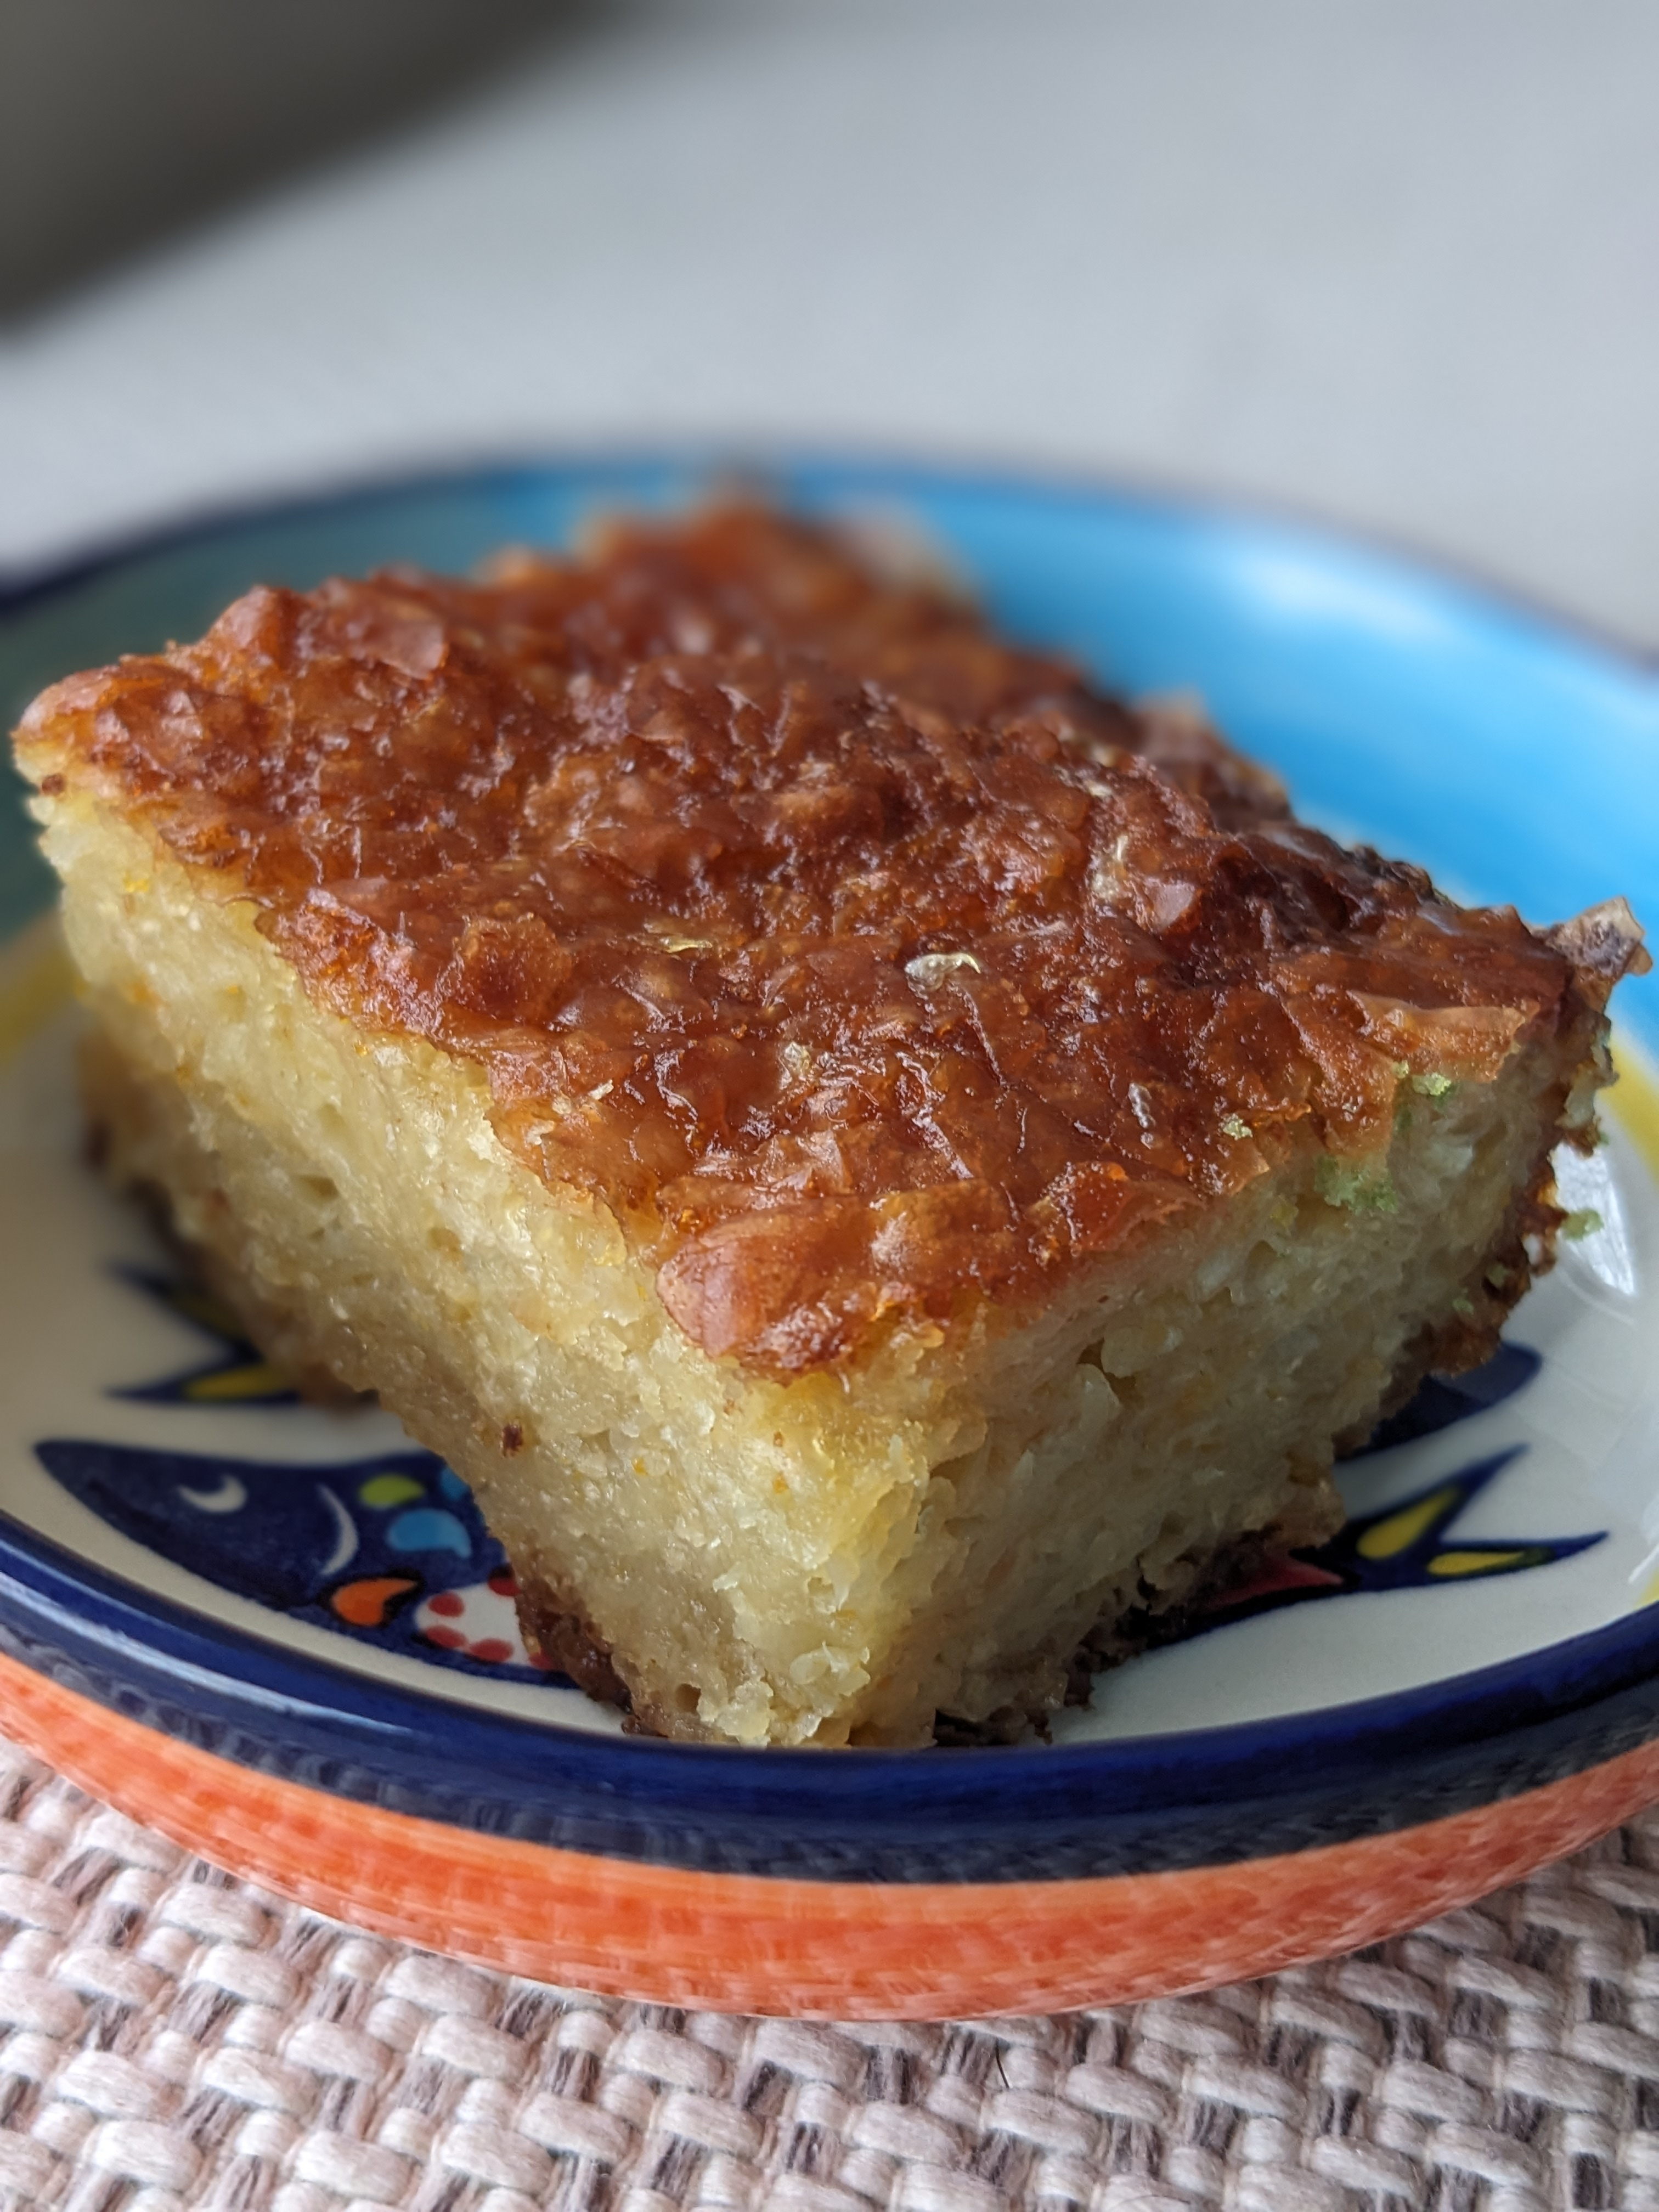
\includegraphics[width=60mm]{monanteras/images/portokalopita.jpg}
\end{figure}
\begin{figure}
  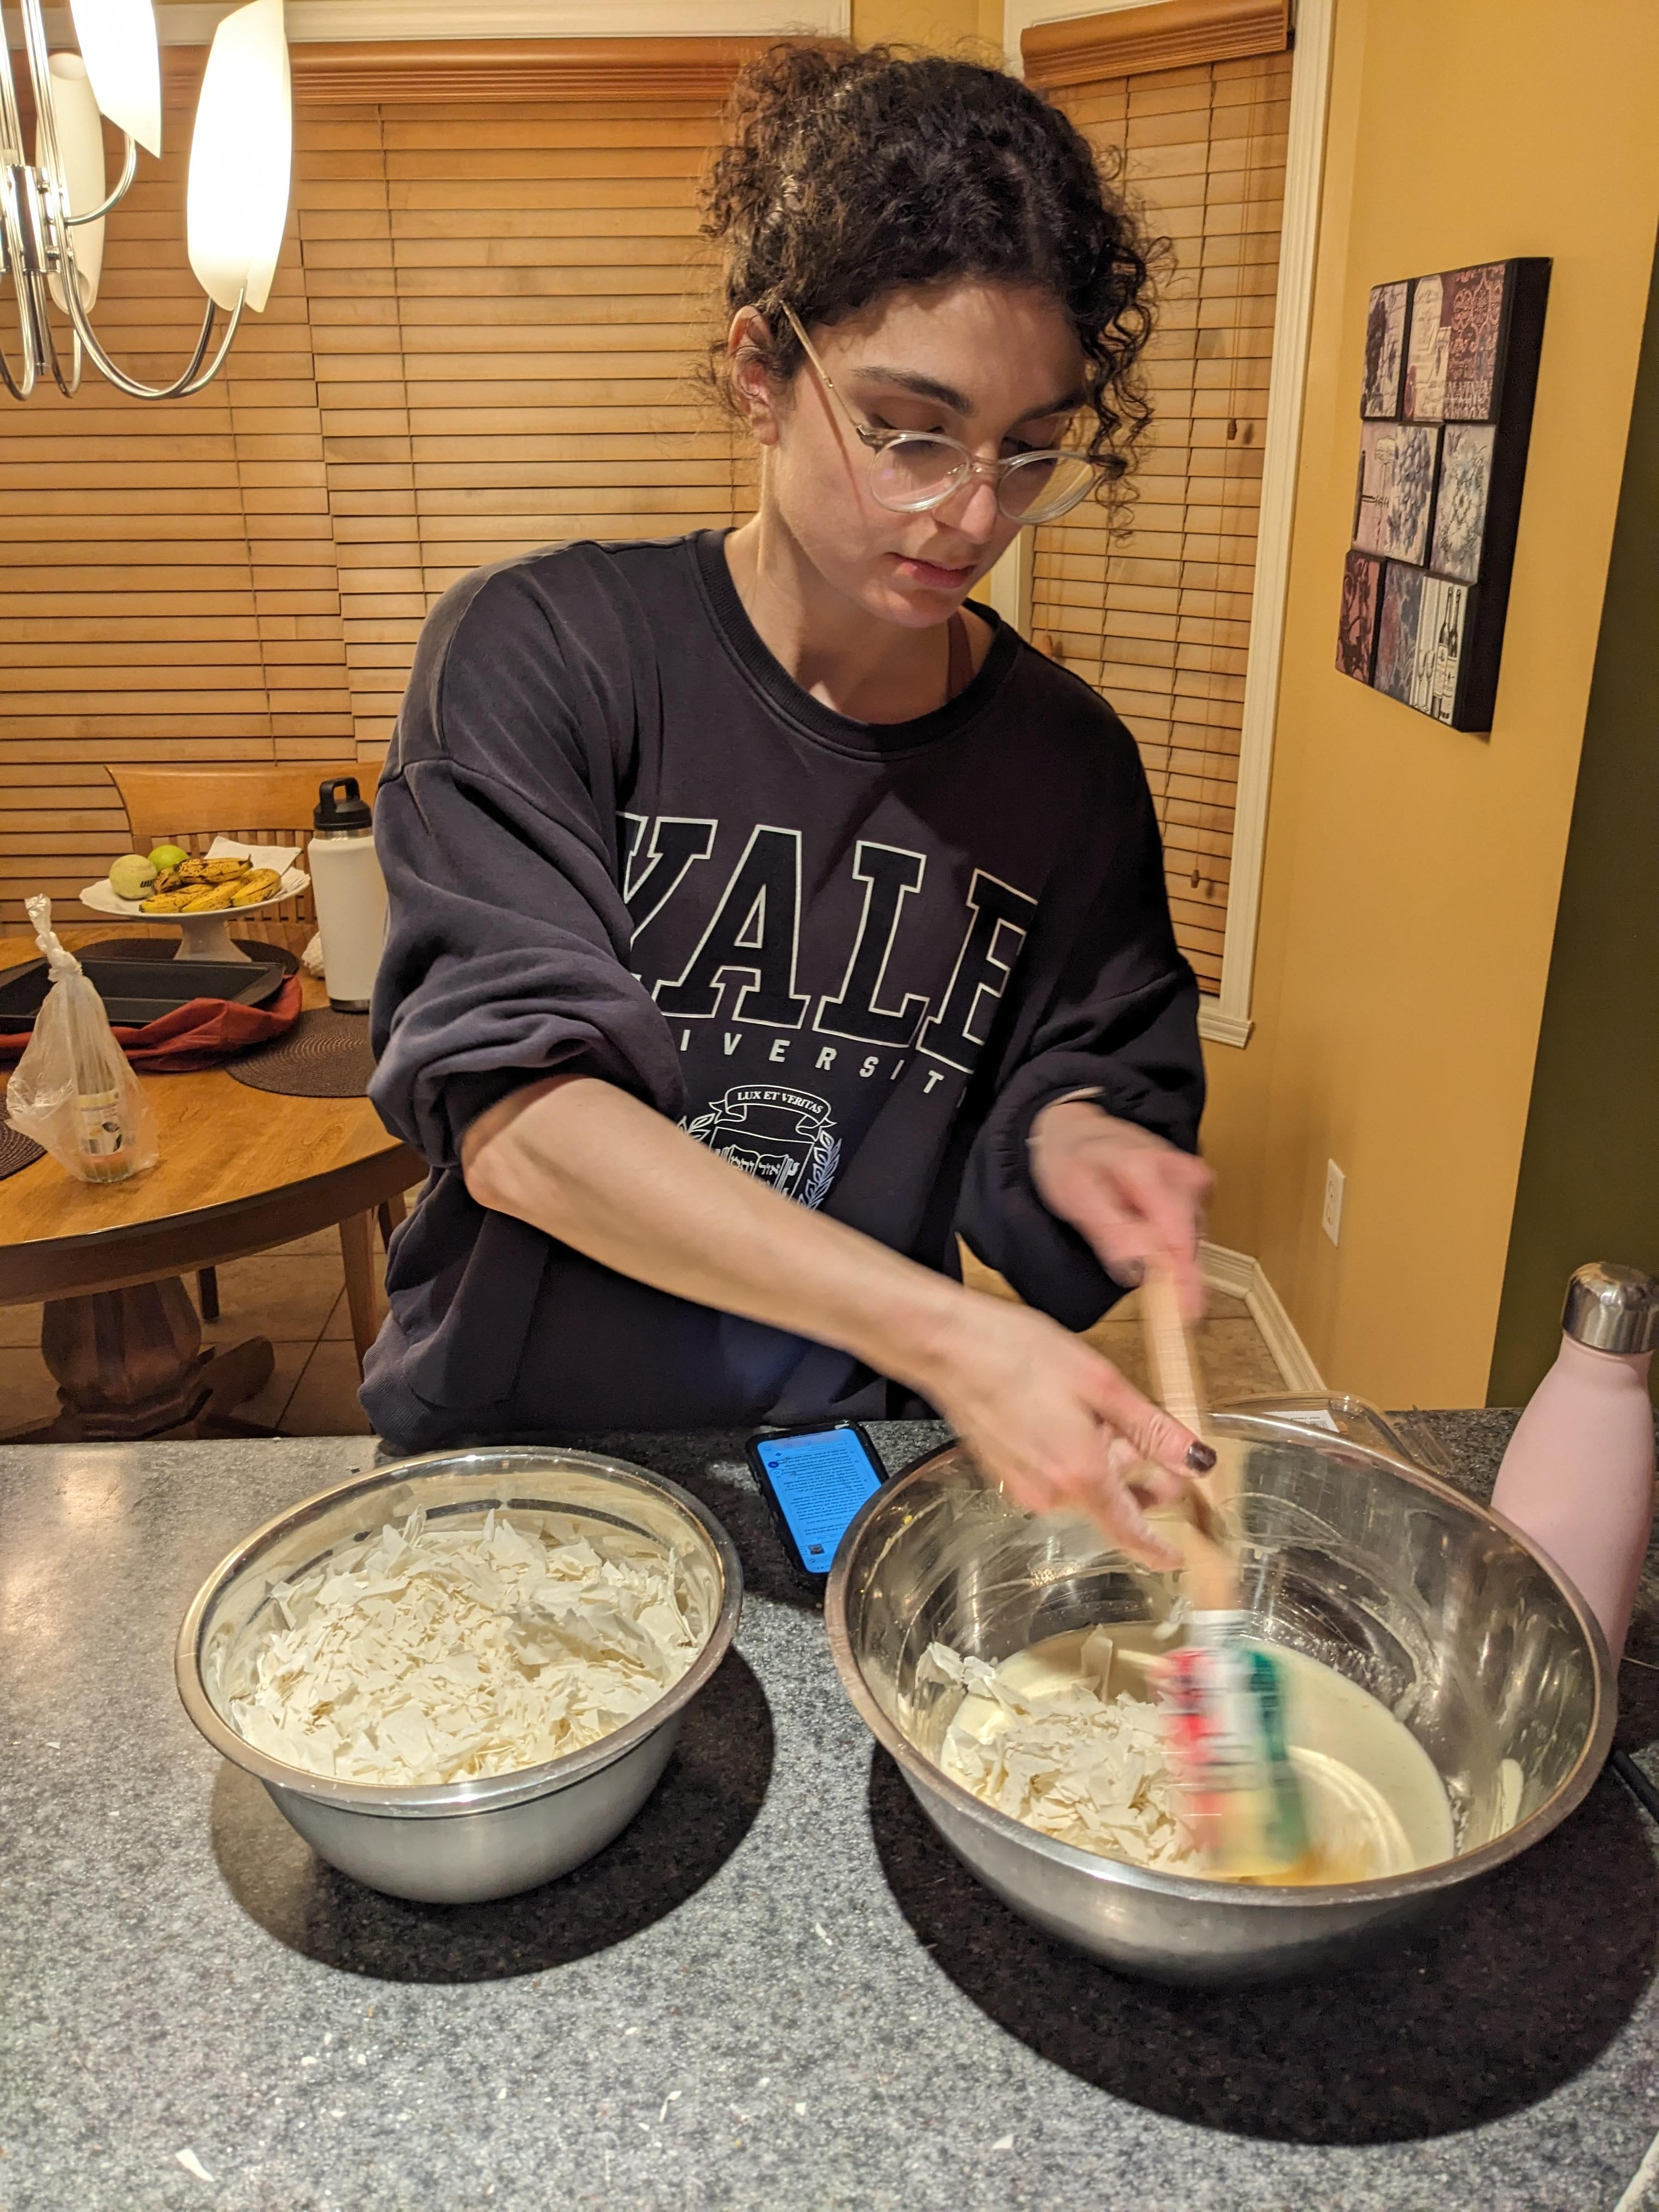
\includegraphics[width=60mm]{monanteras/images/portokalopita2.jpg}
\end{figure}

You can decorate each piece of portokalopita with slices of oranges or keep it simple. Gets better with time :)

